\section{Deformable DETR: Deformable Transformers for End-to-End Object Detection}

\label{appendix:deformable-detr-paper}

\subsection{Overview}

\par Zhu \textit{et al} in their 2021 paper titled \textit{Deformable DETR: Deformable Transformers for End-to-End Object Detection} aims to replace the vanilla dense attention, which is the main computational bottleneck in DETR, with a deformable attention module. This can significantly reduce computational costs and can also improve convergence.
\par

\subsection{Architecture}
\begin{figure}[h]
	\centering
	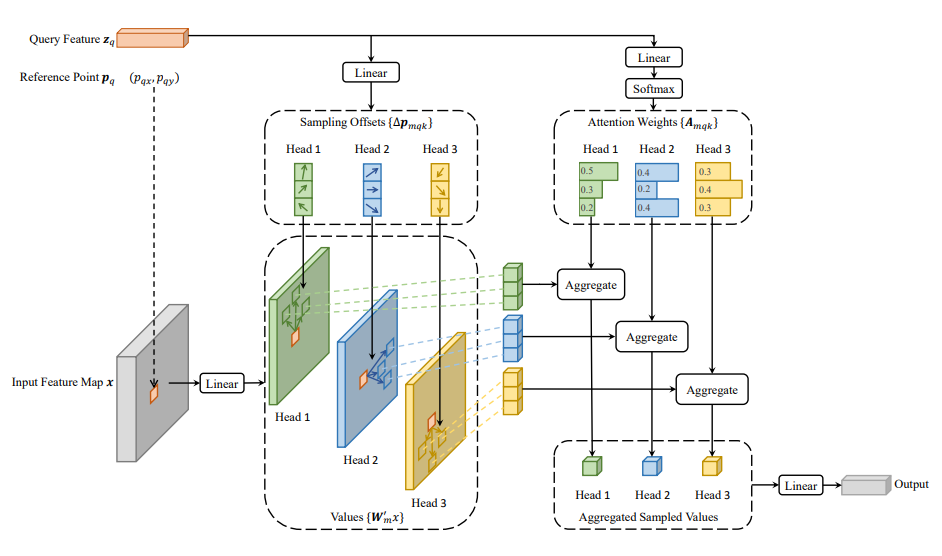
\includegraphics[width=\linewidth]{assets/img/deformable-attention-module.png}
	\caption{Deformable Attention Module by Zhu
		\textit{et al} (Courtesy \cite{zhu2020deformable})}
\end{figure}

\subsubsection{Deformable Attention Module} 
\begin{itemize}
	\item Regardless of the spatial size of the feature maps, it only attends to a small set of key sampling points around a reference point. Convergence and feature spatial resolution issues can be mitigated by assigning only a small fixed number of keys to each query.
	\item Assume an input feature map $x \in R^{C\times H \times W}$ , let q index a query element with content feature zq and a reference point pq, then deformable attention feature is calculated using
	$$ DeformAttn(z_q, p_q, x) = \displaystyle\sum\limits_{m=1}^M W_m
	[\displaystyle\sum\limits_{k=1}^K A_{mqk}\cdot W'_mx(p_q+\Delta p_{mqk})]
	$$
	where k is used to index the sampled keys, m is used to index the attention head of the model, and K is the total sampled key number taken. $\Delta p_{mqk}$ denotes the sampling offset and  $A_{mqk}$ denotes the attention weight of the $k^{th}$ sampling point in the $m^{th}$ attention head, respectively.
\end{itemize}

\subsubsection{Multi-scale Deformable Attention Module}
\begin{itemize}
	\item Deformable attention module can be easily extended for multi-scale feature maps.  
	\item Let $\{{x^l}\}_{l=1}^L$ be the input multi-scale feature maps, where  $x^l \in R^{C\times H^l \times W^l}$ . Let $ \hat p_q \in [0, 1]^2$ be the normalised coordinates of the reference point for each query element q, then the multi-scale deformable attention module is applied by 
	$$DeformAttn(z_q, \hat{p}_q, \{{x^l}\}_{l=1}^L) = 
	\displaystyle\sum\limits_{m=1}^M W_m
	[\displaystyle\sum\limits_{l=1}^L\displaystyle\sum\limits_{k=1}^K A_{mlqk}\cdot W'_mx^l(\phi _l (\hat p_q)+\Delta p_{mlqk})]$$
	
	Where k is used to index the sampling point , l is used to index the input feature level and m is used to index the attention headt. $\Delta p_{mlqk}$ denotes the sampling offset and $A_{mlqk}$ denotes attention weight of the $k^{th}$ sampling point in the $l^{th}$ feature level and the $m^{th}$ attention head of the model.
\end{itemize}

\subsubsection{Deformable Transformer Encoder}
\begin{itemize}
	\item The proposed multiscale deformable attention module replaces the transformer attention modules that process feature maps in DETR.
	\item The input and output of the encoder are both multi-scale feature maps and have the same resolutions.
\end{itemize}	


\subsubsection{Deformable Transformer Decoder}

\begin{itemize}
	\item The decoder includes cross-attention and self-attention modules.
	\item Object queries in the cross attention modules extract features from feature maps, where the key elements are the feature maps which is the output of the encoder. Object queries interact with each other in the self-attention modules, in which the key elements are of the object queries.
	\item In decoder the cross-attention module is replaced with the multi-scale deformable attention module which is mentioned above, while the self-attention modules remain unaltered.
\end{itemize}
\subsection{Conclusion}
\par Zhu \textit{et al} present Deformable DETR, which is an efficient and fast-converging end-to-end object detector. It uses the multi-scale deformable attention modules, which are an efficient attention mechanism in processing image feature maps.